\documentclass[../main.tex]{subfiles}

\begin{document}
%what, why, how
\section{Prototype Implementation: Matplottoy}
\label{sec:implementation}
\begin{figure}[H]
    \begin{subfigure}{0.5\textwidth}
        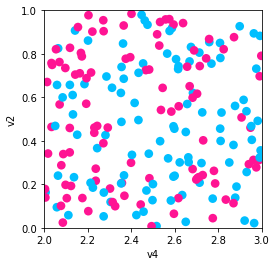
\includegraphics[width=\textwidth]{figures/code/scatter_0.png}
    \end{subfigure}
    \begin{subfigure}{0.5\textwidth}
        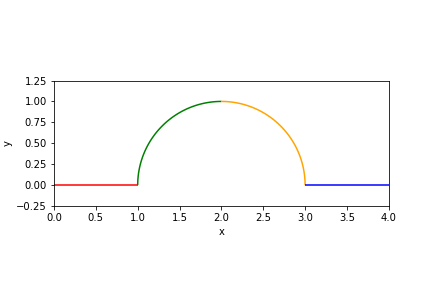
\includegraphics[width=\textwidth]{figures/code/line_1.png}
    \end{subfigure}
    \caption{Scatter plot and line plot implemented using prototype artists and data models, building on Matplotlib rendering.}
    \label{fig:code_scatter_line}
\end{figure}

We implemented a proof of concept of the topological model to demonstrate its feasibility. We implemented the artist classes for the scatter, line, and bar plots shown in figure~\ref{fig:code_scatter_line} because scatter and line have different continuities \gbase\ and visual bundles \vtotal\. We built our prototype on top of the existing Matplotlib architecture \cite{hunterMatplotlib2DGraphics2007,hunterArchitectureOpenSource} so that we can initially focus on the data to graphic transformations and rely on Matplotlib for the rendering. 

To generate figure~\ref{fig:code_scatter_line} in our prototype, we set up a canvas \mintinline{python}{fig} and an axes to draw on \mintinline{python}{ax} and 
\begin{multicols*}{2}
\begin{minted}[linenos]{python}
    fig, ax = plt.subplots()
    artist = Point(table, transforms)
    ax.add_artist(artist)
\end{minted}
\columnbreak
\begin{minted}[linenos]{python}
    fig, ax = plt.subplots()
    artist = Line(table, transforms)
    ax.add_artist(artist)
\end{minted}
\end{multicols*}
 and then pass in \dsection=\mintinline{python}{table} and \vchannel=\mintinline{python}{transforms} into equivalence classes \vartisteq=\mintinline{python}{Point} and  \vartisteq=\mintinline{python}{Line}.  

\subsubsection{Artist Class $\vartist^{\prime}$}
What, why, how>
We implement the \vartist\ functions that transform data to visual representations as the equivalence class of artists such that the user configure the visual sections \vsection\ as a parameter \mintinline{python}{transforms}

\begin{minted}[linenos]{python}
    class ArtistClass(matplotlib.artist.Artist):
        def __init__(self, data, transforms, *args, **kwargs):
            super().__init__(*args, **kwargs)
        def draw(self, renderer, *args, **kwargs):
            super().draw(renderer, *args, **kwargs)
\end{minted}





As mentioned in section~\ref{sec:artist_equivalance}, it would be impractical to implement graph types as \vartist\ functions where all the visual parameters are specified.  

\subsubsection{Encoders \vchannel}
what, why, how?
\subsubsection{Data \dtotal}
what, why, how?

\subsubsection{Case Study: Iris}

\end{document}